\section{Cardinality}
\label{sec:cardinality}

In this chapter the following basic concepts about functions between sets are assumed:

\begin{quote}
  \textsf{function/mapping, domain, target/codomain, range/image, injection/one-to-one, \\ surjection/onto, bijection, identity map, composite.}
\end{quote}
(Words that are separated by a slash are equivalent.)

Let $A, B$ be two sets.
If there is a bijection from $A$ onto $B$ then $A$ and $B$ are said to have \textsf{equal cardinality}, and we hereby write $A \sim B$.
The relation $\sim$ is an equivalence relation, that is,
\begin{itemize}
  \item $A \sim A$.
  \item $A \sim B$ implies $B \sim A$.
  \item $A \sim B \sim C$ implies $A \sim C$.
\end{itemize}
We also write $\operatorname{card} A = \operatorname{card} B$, $\# A = \# B$, or $|A| = |B|$ when $A, B$ have equal cardinality.

\begin{defn}
  A set $S$ is called
  \begin{itemize}
    \item \textsf{finite} if it is empty or for some $n \in \mathbb{N}$ we have $S \sim \{1, 2, \dots, n \}$.
    \item \textsf{infinite} if it is not finite.
    \item \textsf{countable} if $S \sim \mathbb{N}$.
    \item \textsf{at most countable} if it is finite or countable.
    \item \textsf{uncountable} if it is infinite but not countable.
  \end{itemize}
\end{defn}

That $S$ is countable means that there is a bijection $f: \mathbb{N} \to S$, and this gives a way to list the elements of $S$ as $s_1 = f(1)$, $s_2 = f(2)$, $s_3 = f(3)$, etc.
Conversely, if a set $S$ is presented as an infinite list (without repetition) $S = \{ s_1, s_2, s_3, \dots \}$, then it is countable:  Define $f(k) = s_k$ for all $k \in \mathbb{N}$.
In brief, ``countable'' is ``listable.''

We are going to establish two useful facts: $\mathbb{N}, \mathbb{Z}$, and $\mathbb{Q}$ are all countable, but $\mathbb{R}$ is uncountable.
That $\mathbb{N}$ and $\mathbb{Z}$ are countable are easy: using the identity map on $\mathbb{N}$ shows that $\mathbb{N}$ is itself countable, and we may list elements of $\mathbb{Z}$ as
\[
  0, 1, -1, 2, -2, 3, -3, \dots, k, -k, \dots.
\]
In fact, we are going to show first that the set of all {\em positive} rational numbers are countable, then using the trick above to conclude that $\mathbb{Q}$ is also countable.

\begin{prop}
  \label{prop:3-2}
  \begin{enumerate}[(1)]
    \item Any infinite subset $A$ of a countable set $B$ is also countable.
    \item If there is a surjection $f: \mathbb{N} \to B$ and $B$ is infinite then $B$ is countable.
  \end{enumerate}
\end{prop}

\begin{proof}
  \begin{enumerate}[(1)]
    \item After a bijection, we may assume that $B = \mathbb{N}$.
      Let $a_k$ be the $k^{\text{th}}$ smallest number in $A$.
      Then $k \mapsto a_k$ establishes a bijection from $\mathbb{N}$ onto $A$, hence $A$ is countable.

    \item For each $b \in B$ the set $\{k \in \mathbb{N} \colon f(k) = b \}$ is nonempty and hence contains a smallest element; say $h(b) = k$ is the smallest integer that is sent to $b$ by $f$.
      Clearly if $b, b' \in B$ and $b \ne b'$ then $h(b) \ne h(b')$.
      That is, $h: B \to \mathbb{N}$ is an injection which bijects $B$ to $h(B) \subseteq \mathbb{N}$.  Since $B$ is infinite, so is $h(B)$; since $h(B)$ is countable by (1), so is $B$.
  \end{enumerate}
\end{proof}

\begin{prop}
  $\mathbb{N} \times \mathbb{N}$ is countable.
\end{prop}

\begin{proof}
  Define a function $f: \mathbb{N} \times \mathbb{N} \to \mathbb{N}$ as 
  \[
    f(i,j) = \frac{(i+j-1)(i+j-2)}{2} + i, \qquad i, j \in \mathbb{N}.
  \]
  One checks that $f$ is indeed a bijection, therefore $\mathbb{N} \times \mathbb{N}$ is countable.
\end{proof}

\noindent{\em Remark.} Using $f^{-1}$ in the proof above, the elements of $\mathbb{N} \times \mathbb{N}$ are listed in order as
\[
  (1,1), (1,2), (2,1), (1,3), (2,2), (3,1), (1,4), (2,3), (3,2), (4,1), \dots.
\]

\begin{cor}
  \label{cor:3-4}
  The Cartesian product of two countable sets is still countable.
\end{cor}

\begin{thm}
  $\mathbb{Q}$ is countable.
\end{thm}

\begin{proof}
  We are going to show that the set $\mathbb{Q}_{>0}$ is countable.
  After that, the trick from $\mathbb{N}$ to $\mathbb{Z}$ can be applied again to show that $\mathbb{Q}$ is countable.

  Indeed, $\mathbb{Q}_{>0}$ is an infinite set.  The function
  \[
    f(i,j) = \frac{i}{j}, \qquad i, j \in \mathbb{N},
  \]
  is a surjection from $\mathbb{N} \times \mathbb{N}$ onto $\mathbb{Q}_{>0}$.
  Therefore $\mathbb{Q}_{>0}$ is countable by (2) in Proposition~\ref{prop:3-2}.
\end{proof}

\begin{cor}
  For each $m \in \mathbb{N}$ the set $\mathbb{Q}^m$ is countable.
\end{cor}

\begin{proof}
  Use Corollary~\ref{cor:3-4} and mathematical induction sufficiently many times.
\end{proof}

Unlike $\mathbb{Q}$, the cardinality of $\mathbb{R}$ behaves completely different.

\begin{thm}
  $\mathbb{R}$ is uncountable.
\end{thm}

\begin{proof}
  There are other proofs of the uncountability of $\mathbb{R}$, but none so beautiful as this one, which was due to Cantor.
  It is assumed here that each real number $x$ has a decimal expansion $x = N.x_1x_2x_3\dots$, and it is uniquely determined by $x$ except for $x = \dfrac{K}{10^n}$ with $K \in \mathbb{Z}, n \in \mathbb{Z}_{\geqslant 0}$ (there are two in this case.)
  
  Assume the contrary, i.e. $\mathbb{R}$ is not uncountable.
  Being infinite, $\mathbb{R}$ must then be countable.
  Hence there is a bijection $f : \mathbb{N} \to \mathbb{R}$.
  Using $f$, we list the elements of $\mathbb{R}$ along their decimal expansions as an array, and consider the digits $x_{ii}$ that occur along the diagonal in this array, see below.

  \begin{figure}[t]
    \centering
    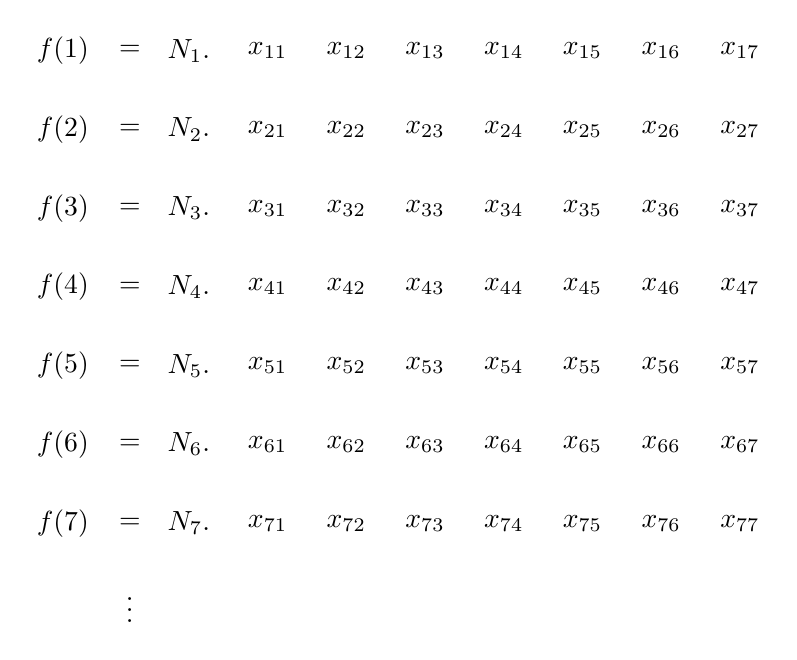
\begin{tikzpicture}
      \foreach \x in {1,2,3,4,5,6,7}
      {\node at (0, -\x) {$N_{\x}.$};
	\node at (-0.75,-\x) {$=$};
       \node at (-1.6,-\x) {$f(\x)$};
      }
      \foreach \x in {1,2,3,4,5,6,7}
        \foreach \y in {1,2,3,4,5,6,7}
	  \node at (\y, -\x) {$x_{\x\y}$};
      \node at (-0.75,-8) {$\vdots$};
    \end{tikzpicture}
  \end{figure}

  For each $i$, choose a digit $y_i$ such that $y_i \ne x_{ii}$ and $y_i \notin \{0,9\}$.  Then the number $y = 0.y_1y_2y_3\dots$ does not appear in the list of all elements of $\mathbb{R}$, which is a contradiction!
\end{proof}

\begin{cor}
  The (non-degenerate) intervals $(a,b)$ and $[a,b]$ are both uncountable. 
\end{cor}
